\section{Drawing the Polygonal Dual}
\label{sect:drawing-the-dual}

In the second step of the pipeline, we apply a force-directed graph drawing algorithm to the initial map graph $G_\text{init}$ produced by \cref{alg:transformation-to-dual} to generate the approximately area-proportional map graph $G_\text{prop}$.

In a force-directed algorithm, we interpret a graph's vertices as particles in a physical system.
Based on the structure of the graph and the relative position of the particles, we define several forces that act to bring the system to a stable equilibrium position in which its potential energy is at a local minimum.
In these equilibrium positions, the system is in a somewhat relaxed state that, in the context of graph drawing, generally is a visually appealing drawing of the graph.
We find an equilibrium position by iteratively computing the net force acting on each particle and displacing it by a small amount in the direction of the net force, based on its absolute value.



\paragraph{Forces}

We define the forces that exist in our particle system with two goals in mind:
First, the faces of the graph (the regions of the map) to have an area ought to be close to proportional to some prescribed value.
Second, we want the faces to be \emph{locally fat}.
Our intuitive understanding of local fatness is that a region shouldn't have drawn-out, tight corridors.
We formalize and discuss different quantifiable measures that aim to capture the local fatness of regions in \cref{chap:evaluation}.
Note that both of these are soft requirements.
Planarity of the resulting drawing, on the other hand, is a hard requirement that must be preserved at all costs.

Let us now discuss the concrete force components that act to bring our particle system to an equilibrium position.
%
\begin{itemize}
\item \textbf{Air Pressure:} % alam2013computing
Motivated by Alam \etal{} \cite{alam2013computing}, we treat the polygonal regions as volumes of some amount of air equal to the respective face's weight.
This allows us to define an analog to air pressure in the polygonal regions that exerts forces on the regions' edges.
This force is responsible for growing faces that are currently compressed and shrinking faces that are currently larger than they should be, therefore working towards the statistical accuracy of the generated map.

We want this force and the overall drawing to be agnostic to constant factors of the face weights and therefore compute the normalized pressure $P(f)$ in an internal face $f$ as
%
\begin{equation*}
	P(f) \coloneqq \frac{w(f)}{A(f)} \cdot \frac{\sum_{g \in F}{A(g)}}{\sum_{g \in F}{w(g)}},
\end{equation*}
%
where $A(f)$ is the area currently covered by some internal face $f$ and $w(f)$ its weight.
We set the normalized pressure in the outer face to the weighted average normalized pressure, \ie{}
%
\begin{equation*}
	P(f_\text{outer}) \coloneqq \frac{\sum_{f \in F}{A(f) \cdot P(f)}}{\sum_{f \in F}{A(f)}} = 1.
\end{equation*}

Physical pressure is the ratio of force to area.
The air pressure in each of the regions $f$ therefore exerts a force on each bounding edge $e = \{u,v\}$ based on the pressure's magnitude and the edge's length $l(e)$ in relation to the entire region's boundary's length $l(f)$.
We orient $e = \{u,v\}$ such that $u$ directly precedes $v$ on the boundary of $f$ and define the force as
%
\begin{equation}
	\vec{F}_P((u,v);f) \coloneqq
	3 \cdot P(f)\cdot\frac{l(e)}{l(f)}
	\cdot \Norm(\Perp(\longvec{vu}))
	,
\end{equation}
%
where $\Perp(\cdot)$ rotates a vector by $90^\circ$ in counterclockwise direction and $\Norm(\cdot)$ normalizes a vector to unit length.
We apply $\vec{F}_P(\{u,v\};f)$ to both endpoints $u$ and $v$ of the edge, as illustrated in \cref{fig:drawing-forces-air-pressure}.

\begin{figure}[H]
	\centering
	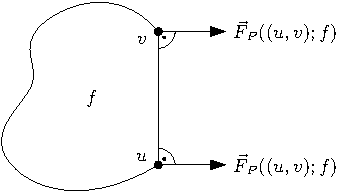
\includegraphics[height=35mm]{Resources/Drawing-Forces-AirPressure.pdf}
	\caption{Forces exerted on the endpoints of the edge $e = \{u,v\}$ by the air pressure in the region $f$.}
	\label{fig:drawing-forces-air-pressure}
\end{figure}

Considering every edge is incident to exactly two faces, we can write the net force exerted on an oriented edge $e = (u,v)$ incident to face $f$ on the left and face $g$ on the right as
%
\begin{equation*}
	\vec{F}_P((u,v);f,g) \coloneqq
	3 \cdot \left( P(g)\cdot\frac{l(e)}{l(g)} - P(f)\cdot\frac{l(e)}{l(f)} \right)
	\cdot \Norm(\Perp(\longvec{uv}))
	,
\end{equation*}
%
matching the force that Alam \etal{} \cite{alam2013computing} use for computing their cartograms.


\item \textbf{Angular Resolution:} % argyriou2013maximizing
Internal face angles close to $0^\circ$ cause tight corridors in the form of pointy spikes and angles close to $360^\circ$ the opposite \emdash{} both features we want to avoid if possible.
We therefore define a force that optimizes angular resolution, \ie{} a force that tries to evenly distribute the angles formed by the incident edges around a vertex $v$ at $\frac{360^\circ}{\deg(v)}$ each.

Let $v$ be a vertex and let $u$ and $w$ be two successive neighbors of $u$ in counterclockwise order.
Also let $\measuredangle_{uvw} \in \lbrack 0^\circ, 360^\circ )$ denote the normalized angle from $u$ via $v$ to $w$ measured in counterclockwise direction.
With this, we define the force $\vec{F}_\measuredangle(v;u,w)$ as
%
\begin{equation}
	\vec{F}_\measuredangle(v;u,w) \coloneqq
	\frac{1}{2} \cdot \frac{\frac{360^\circ}{\deg(u)} - \measuredangle_{uvw}}{\measuredangle_{uvw}}
	\cdot \Bsc(\angle_{uvw})
	.
\end{equation}

Here $\Bsc(\angle_{uvw})$ computes the normalized bisector of the given angle, \ie{} $\Norm(\longvec{vu})$ rotated by $\frac{1}{2} \measuredangle_{uvw}$ in counterclockwise direction.
The construction of $\vec{F}_\measuredangle(v;u,w)$ is illustrated in \cref{fig:drawing-forces-angular-resolution}.

\begin{figure}[H]
	\centering
	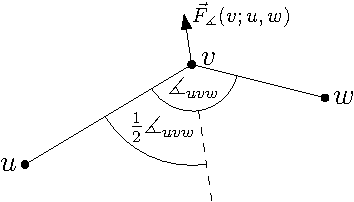
\includegraphics[height=40mm]{Resources/Drawing-Forces-AngularResolution.pdf}
	\caption{Force exerted on some vertex $v$ with successive neighbors $u$ and $w$ of $v$ where $\measuredangle_{uvw} > \frac{360^\circ}{\deg(v)}$.}
	\label{fig:drawing-forces-angular-resolution}
\end{figure}

For all triplets $(u,v,w)$ of vertices $v$ and successive neighbors $u$, $w$ of $v$, we apply $\vec{F}_\measuredangle(v;u,w)$ to $v$.
If the angle at $v$ is currently too small, the force acts to move $v$ along the bisector, thereby increasing the angle; otherwise it acts to move $v$ against the bisector, thereby decreasing the angle.

Argyriou \etal{} \cite{argyriou2013maximizing} use a similar force to obtain uniform angles around all vertices.
However, instead of applying the force to the vertex $v$ whose angular resolution we want to improve as we do, they apply perpendicular forces to its neighbors.
In our tests, the approach of Argyriou \etal{} has shown not to converge well due to us not having a force acting towards a uniform edge length, as discussed below in a bit.


\item \textbf{Vertex-vertex repulsion:} % eades84heuristic
We define a repulsive force between pairs of vertices to prevent the vertices from clumping together.
This is important because in order to preserve planarity, vertices that are very close to others will need to have their movement restricted severely, possibly hindering us from satisfying our aesthetic criteria.
We think of the vertices as charged particles that push each other away and define a repulsive force based on Coulomb's law that is exerted along the line connecting pairs of vertices and whose magnitude depends on their Euclidean distance:
%
\begin{equation}
	\vec{F}_\leftrightarrow(u;v) \coloneqq
	25 \cdot \frac{1}{\norm{\longvec{uv}}^2}
	\cdot \Norm(\longvec{uv})
\end{equation}

For pairs $(u, v) \in V^2, u \neq v$, we apply $\vec{F}_\leftrightarrow(u;v)$ to $u$.
We restrict ourselves to pairs $(u,v)$ where $u$ and $v$ lie together on the boundary of some face for performance reasons and because for other pairs, there'd be other vertices or edges between $u$ and $v$ that would push the two vertices apart.

This kind of force was first used by Eades \cite{eades84heuristic}, albeit only for non-adjacent pairs of vertices.
We apply this force to adjacent vertices as well because we don't use spring-like forces between adjacent vertices trying to achieve a uniform edge length (and therefore some non-zero distance) as Eades does, as discussed below.


\item \textbf{Vertex-edge repulsion:} % bertault1999force
In another attempt to prevent tight corridors from forming, we define an additional repulsive force between vertices and edges.
Given an edge $e = \{u,w\}$ and non-incident vertex $v$, we define $v_+$ as the point on the segment from $u$ to $w$ with the smallest Euclidean distance to $v$.
We then define the repulsive force as
%
\begin{equation}
	\vec{F}_\bot(v;\{u,w\}) \coloneqq
	10 \cdot \frac{1}{\norm{\longvec{v_+v}}^2}
	\cdot \abs{\vec{n}_e \cdot \Norm(\longvec{v_+v})}
	\cdot \Norm(\longvec{v_+v})
	,
\end{equation}
%
where $\vec{n}_e$ is the normalized normal vector of the edge $e$ pointing in either direction.
The following figure illustrates the construction of the force $\vec{F}_\bot(v;\{u,w\})$:
%
\begin{figure}[H]
	\centering
	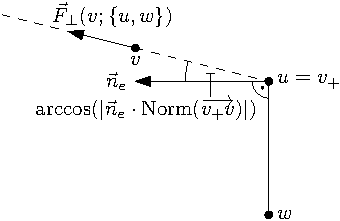
\includegraphics[height=40mm]{Resources/Drawing-Forces-VertexEdgeRepulsion.pdf}
	\caption{Force exerted on some vertex $v$ by a non-incident edge $\{u,w\}$.}
	\label{fig:drawing-forces-vertex-edge-repulsion}
\end{figure}

Analogous to the vertex-vertex-repulsion discussed above, we compute the force $\vec{F}_\bot(v;\{u,w\})$ only for vertices and edges that lie together on the boundary of some face and apply it to $v$.

This repulsive force is very similar to what Bertault uses in PrEd \cite{bertault1999force}.
However, we have an additional dot product term for how $v$ is positioned relatively to the edge $\{u,w\}$ whereas Bertault drops the force altogether if the orthogonal projection of $v$ onto the line through $u$ and $w$ doesn't lie between $u$ and $w$.
In our tests, Bertault's definition resulted in very unstable simulations as these force swayed back and forth between having full impact and no impact at all.
\end{itemize}

The constant factors of the force components above were determined experimentally and yielded good results for a variety of randomly generated graphs.

Note that we do not define attractive forces between adjacent vertices as most traditional force-directed algorithms do.
Such an attractive force is generally used to keep adjacent vertices close together while nonadjacent vertices are pushed further apart by the repulsive forces.
This works for many graph drawing algorithms because for them, uniform edge length is a desired feature in equilibrium.
In our case, however, there is no correlation between the extent of a region and the number of edges on its boundary and, subsequently, the length of the edges on its boundary.
Including such an attractive force here would in fact be counterproductive.

To make sure that the physical simulation converges, we cool the particle system down over time.
We define a global cooling parameter $\alpha = 0.01$ and, at step $i$ of the iterative process, add $(1 - \alpha)^i$ as a factor to all of the forces mentioned above.
By doing so, we prevent unstable oscillations around equilibrium.

In our implementation, we also smooth vertices of degree 2 that become too close to other vertices and subdivide edges that become too long in order to create more degrees of freedom in the respective face's shape.
To do so, we first compute the average edge length $\bar{l}$ as
%
\begin{equation*}
	\bar{l} \coloneqq \frac1{\abs{E}} \cdot \sum\limits_{e \in E} l(e)
	.
\end{equation*}
%
Then, at each iteration, we subdivide edges that are longer than $2\bar{l}$ at their midpoint and smooth vertices whose distance to the closest other vertex is $\frac{1}{10}\bar{l}$ or less if we can do so without introducing edge crossings.



\paragraph{Preserving Edge Crossing and Combinatorial Properties}

When iteratively displacing the map graph's vertices according to the forces defined above, we must pay close attention to not accidentally introduce edge crossings or change the cyclic order of incident edges around the vertices.

To do so, we adopt the rules of ImPrEd \cite{simonetto2011impred} that ensure no edge crossings are created.
At each step of the algorithm, ImPrEd computes the maximum distance each of the vertices is allowed to move such that the drawing's edge crossing properties are guaranteed to be preserved.
The maximum displacement per vertex is computed in eight general directions, zones of $45^\circ$ each.
The actual displacement of the vertices is then clamped at the maximum distance the vertex can safely move in the desired direction.

As a byproduct, these rules also ensure that the cyclic order of incident edges around the vertices stays the same, thereby preserving the map's combinatorial properties.
